%!TEX root = ../../paper.tex

% Ferdosi 2, MBE
\begin{subfigure}{0.33\textwidth}
	\centering
	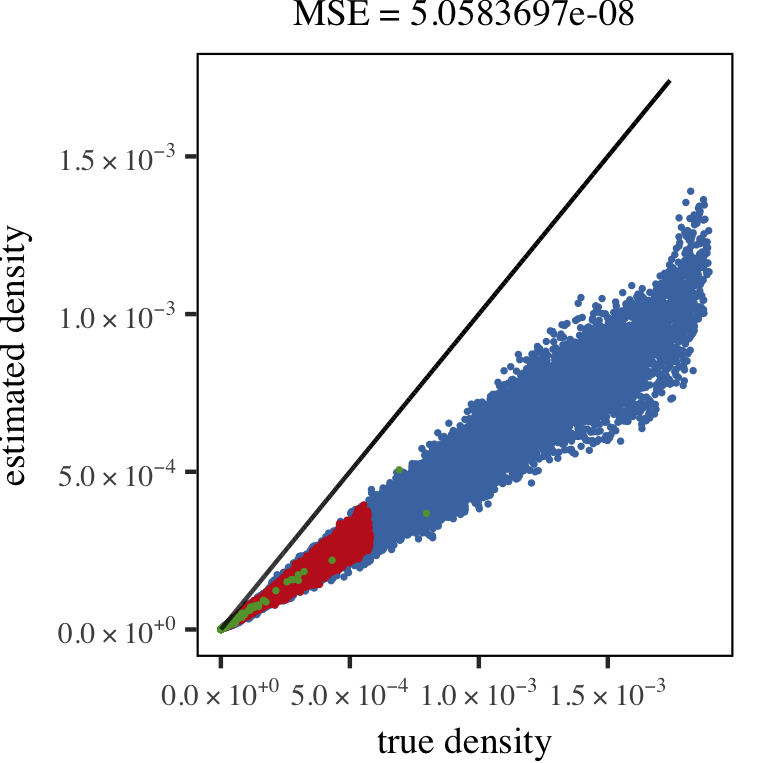
\includegraphics[keepaspectratio=true, width=\textwidth, height=0.185\textheight]{result/img/results_ferdosi_2_60000_mbe_silverman}
	\caption{Set \ferdosiTwo, \mbe}
	\label{fig:results:multisphere:mbe:ferdosi2}
\end{subfigure}
% Baakman 2, MBE
\begin{subfigure}{0.33\textwidth}
	\centering
	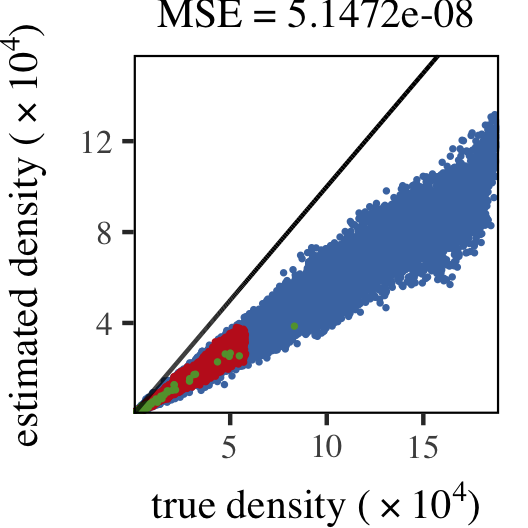
\includegraphics[keepaspectratio=true, width=\textwidth, height=0.185\textheight]{result/img/results_baakman_2_60000_mbe_silverman}
	\caption{Set \baakmanTwo, \mbe}
	\label{fig:results:multisphere:mbe:baakman2}
\end{subfigure}
\subfigvspace
% Ferdosi 2, SAMBE
\begin{subfigure}{0.33\textwidth}
	\centering
	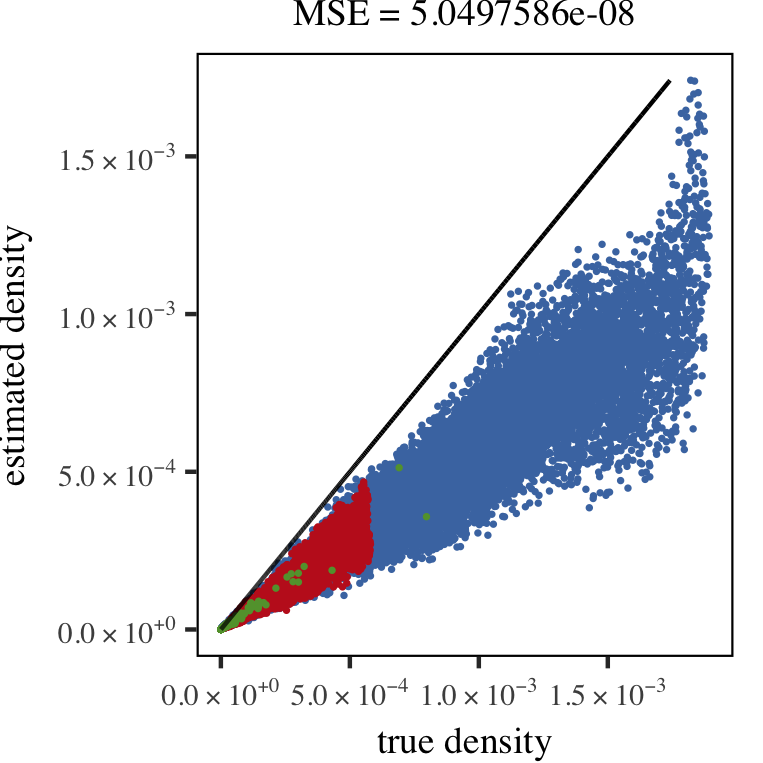
\includegraphics[keepaspectratio=true, width=\textwidth, height=0.185\textheight]{result/img/results_ferdosi_2_60000_sambe_silverman}
	\caption{Set \ferdosiTwo, \sambe}
	\label{fig:results:multisphere:sambe:ferdosi2}
\end{subfigure}
% Baakman 2, SAMBE
\begin{subfigure}{0.33\textwidth}
	\centering
	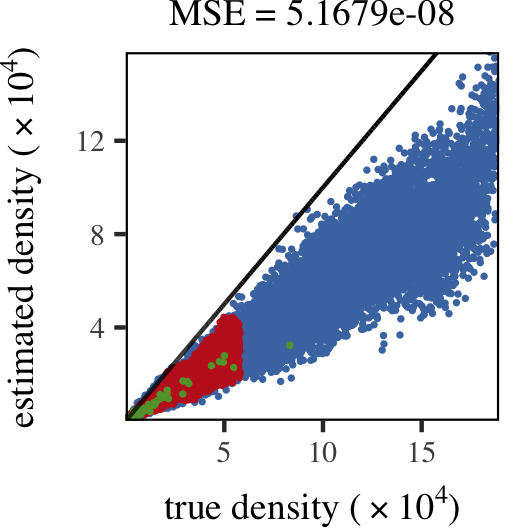
\includegraphics[keepaspectratio=true, width=\textwidth, height=0.185\textheight]{result/img/results_baakman_2_60000_sambe_silverman}
	\caption{Set \baakmanTwo, \sambe}
	\label{fig:results:multisphere:sambe:baakman2}
\end{subfigure}